\documentclass[11pt]{article} %{{{

\usepackage{amsmath}
\usepackage{amssymb}
\usepackage{graphicx}
\usepackage{url}
\usepackage[usenames,dvipsnames,svgnames,table]{xcolor}
\definecolor{light-gray}{gray}{0.8}
\def \del #1{ {\color{light-gray}{#1}} }
\def\yy#1{\footnote{\color{red}\textbf{#1 -YY}} }
\def\ej#1{\footnote{\color{blue}\textbf{#1 -EJ}} }
\usepackage{hyperref}


\usepackage[backend=bibtex]{biblatex}
\addbibresource{main.bib}
\graphicspath{ {./figs} }

\usepackage{array}
\usepackage{subcaption}
%}}}

\begin{document} %{{{

\title{Creativity and Popularity of Fanfictions in Fandoms} %{{{
\date{\today}
\maketitle %}}}

\section{Introduction} %{{{
\label{sec:introduction}
Many creative cultural products in human history are centered around a common topic and developed into different versions through time and interaction between creators. Myths and folktales in oral traditions of civilizations around the world often follow this pattern, for example, the tale of the \emph{Little Red Riding Hood} originated in the 10th century, and has developed multiple variations\cite{littlered}. The legends like \emph{Mahabharata} and \emph{Iliad} also fit with this pattern.

In the contemporary pop culture, this tradition is sometimes found in a new form --- fan works. Sometimes defined more formally as transformative works, they are creative works made by fans based on one or more original works, and are often centered around certain characters or story lines\cite{wiki:transf_work}. For example, a story written by a contemporary fan about Sherlock Holmes in his retirement is considered a fan work. Although fan works contain multiple media types such as art, music and games, one of the most common type is creative writing---fanfictions. People interested in such activities often connect and interact with each other, forming communities known as fandoms\cite{wiki:fandom}.

Similar to other creative works, fanfictions are constantly under selection and evaluation of their readers. The most successful fanfictions may be published and even adapted into other media forms (for example, \emph{Fifty Shades of Grey} was originally a fanfiction of \emph{Twilight}). Meanwhile, the majority of them remain mostly unknown.

We study the creativity and popularity of fanfictions in fandoms using data from Archive of Our Own (AO3). This site hosts fan works --- mainly fanfictions --- that users upload and their metadata, and categorizes them based on fandoms. Established in 2010, it has become one of the most popular transformative work archives. We first show that the creativity of fanfictions has a negative effect on their popularity -- the more a fiction is different from other fictions, the less it is liked by its readers. Then we show that this negative relation influences how authors create fictions: over time, the average distance between fictions become smaller. (Do we really have this result?)

%}}}

\section{Results} %{{{
\label{sec:results}

%}}}



\section{Methods} %{{{
\label{sec:methods}

%}}}

\subsection{Data}
We collected fanfictions from 50 fandoms according to AO3's list of most popular fandoms as of March 2016 \footnote{from this list: \url{http://archiveofourown.org/media}}. To avoid duplication, we remove fandoms with heavy overlapping (e.g.: we keep \emph{Marvel} and removed \emph{Marvel movies}). Fandoms that cover diverse topics (e.g.\emph{k-pop}) are also removed. Finally, we only kept the fictions written in English. This leaves us with 904,760 fictions from 25 fandoms. The number of fictions in each fandom is shown in Figure \ref{fig:fandom_size}.

\begin{figure}[htbp]
\begin{center}
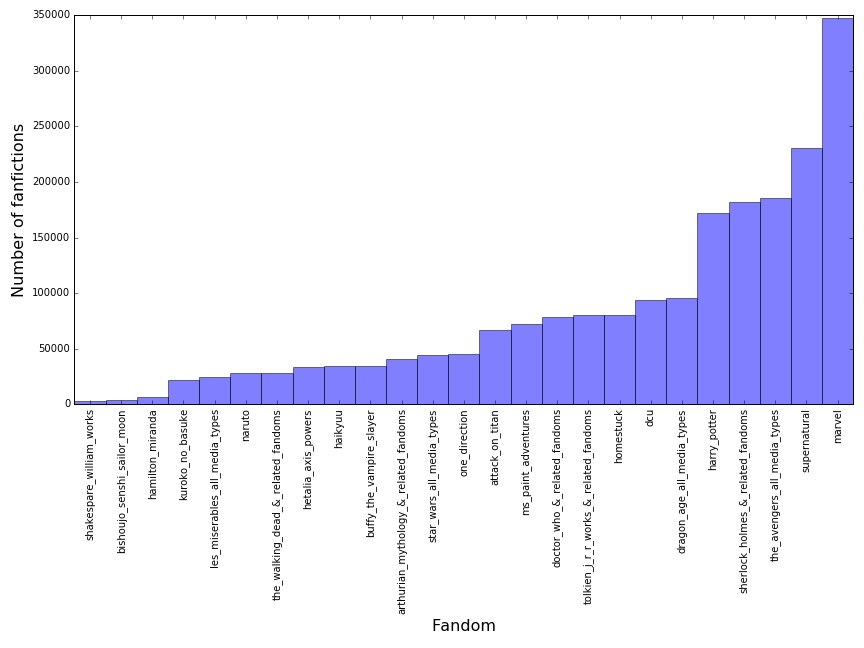
\includegraphics[width=0.9\textwidth]{/fandom_size.png}
\caption{Number of fanfictions in each fandom}
\label{fig:fandom_size}
\end{center}
\end{figure}


Besides the work texts, we also collected metadata including 23 fields. We only used information contained in some of these fields. Table \ref{tab:metadata} gives the names and descriptions of these fields. 

\begin{table}[htp]
\caption{Metadata of the writings}
\begin{center}
\begin{tabular}[width=0.8\textwidth]{p{2cm}|p{3cm}|p{5cm}}
  \hline			
 Fields & Description & Usage\\ 
   \hline			
Text & The fiction texts. & All text analysis are carried out on these texts.\\
Title & Titles of the fictions. & Used to identify the fictions. \\
Fandoms & Describes which fandom(s) the fiction belongs to. & Used to categorize the fictions.\\
Author & The author of the fiction. & Used for identifying the fictions and for text analysis. \\
Hits & The number of times a fiction is clicked on. & A metric for evaluating the fiction's popularity. \\
Kudos & The number of times that readers "like" the fiction. &  A metric for evaluating the fiction's popularity.\\
Publish Date & The date the fiction was published. & Used to determine the time period that the fiction belongs to.\\
\hline
\end{tabular}
\end{center}
\label{tab:metadata}
\end{table}%

Among the metadata fields, we're especially interested in the fields ``Hits" and ``Kudos", which shows how many times a fiction has been clicked or liked by readers. These are useful proxies for the popularity of a piece of work in a specific fandom.
Both statistics have power-law-like distribution, as shown in  Figure \ref{fig:long_tail}, proving our conception that the popularity of fictions is very imbalanced: most fictions are rarely read and receive little Kudos, while very few get the majority of views and Kudos.

\begin{figure}[htbp]
\begin{center}
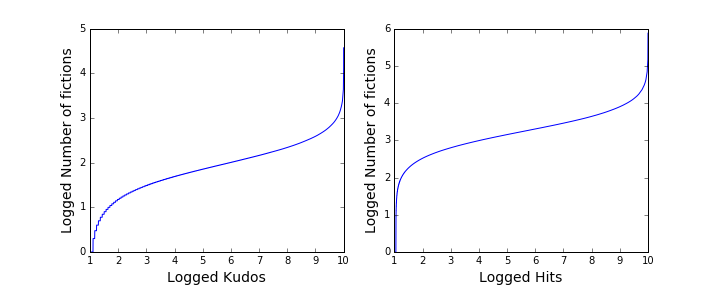
\includegraphics[width=\textwidth]{/kudos_hits_dist.png}
\caption{Log-log CCDF of the distribution of Kudos and Hits. Both follows long-tail distributions, meanwhile, the curve of 
Kudos is steeper, indicating there are more fictions that receive little or no Kudos, while the curve of Hits is smoother. }
\label{fig:long_tail}
\end{center}
\end{figure}

\subsection{Language model}
We model the fictions with a unigram language model. The Good-Turing smoothing\cite{gales1995good} is applied to assign non-zero probabilities to previously unseen unigrams. When creating the unigram list, we also remove the rare unigrams that appear in less than 5 documents.

This transformation allows us to apply many text analysis methods. We choose to use the Kullback--Leibler divergence to measure the distance between texts. Under this measurement, fictions from the same author are more similar and have a smaller KL divergence between each other, compared to fictions from different authors, as shown in Figure \ref{fig:kl_validation}.

\begin{figure}[htbp]
\begin{center}
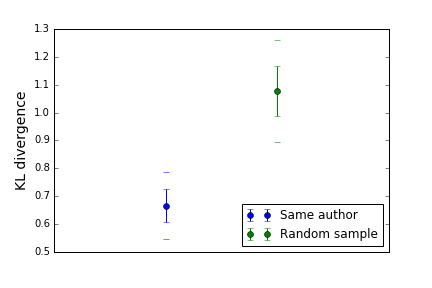
\includegraphics[width=0.6\textwidth]{/kl_validation.png}
\caption{KL divergence between fictions from the same author and fictions from different authors in the Shakespeare fandom. The blue point: The average KL divergence of fictions from same authors. KL divergence of fictions from each author is calculated as the average KL divergence between each pair of her fictions. The green point: The computation repeated on random examples with the same size. The error bars are computed with the bootstrap resampling method. }
\label{fig:kl_validation}
\end{center}
\end{figure}

We further define the concept of a \emph{typical} fiction. A typical fiction of a time period is the average of probability distributions of all fictions in that time period (a month in this study). This allows us to calculate the KL divergence between any fiction and the typical fiction. We then attempt to analyze the relation between a fiction's distance to the typical fiction and the Kudos or Hits that it receives. Because of the long-tailed distribution of Kudos and Hits as described above, log-transformation is applied to the two statistics to balance out this effect. 
% Reorganize and discuss on kudos/hits/distribution
 
Figure \ref{fig:kl_fields} shows a overall descending pattern in Kudos and Hits when KL divergence increases, with the exception of two fandoms ``original work" and ``shakespeare works". It is also interesting to consider ``original work", because as s specific category in AO3, it contains original stories instead of fanfictions. Its standing out indicated that the other fandoms may indeed have some behavior in common. 

\subsection{Regression}




\begin{figure*}[t!]
    \centering
    \begin{subfigure}[t]{0.7\textwidth}
        \centering
        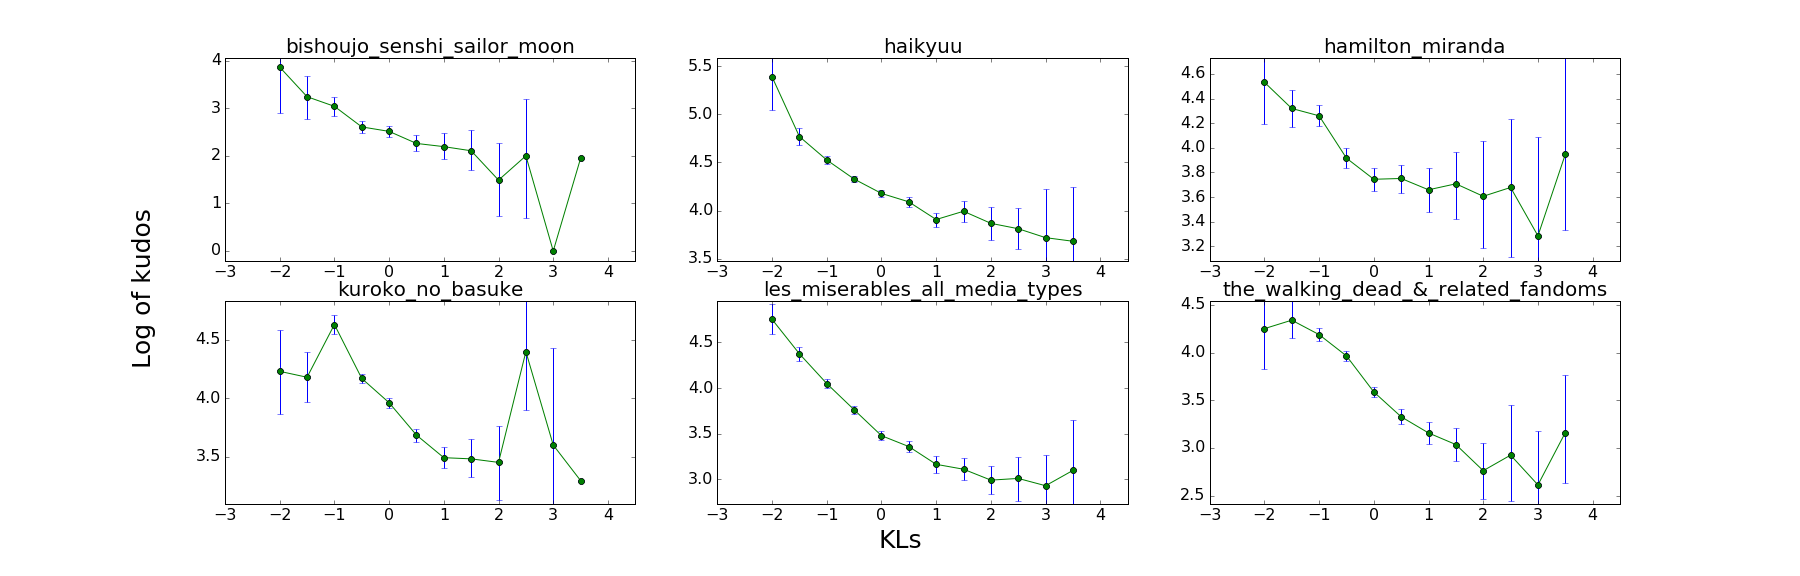
\includegraphics[height=7in]{/kl_kudos.png}
        \caption{Kudos}
    \end{subfigure}%
    ~ 
    \begin{subfigure}[t]{0.3\textwidth}
        \centering
        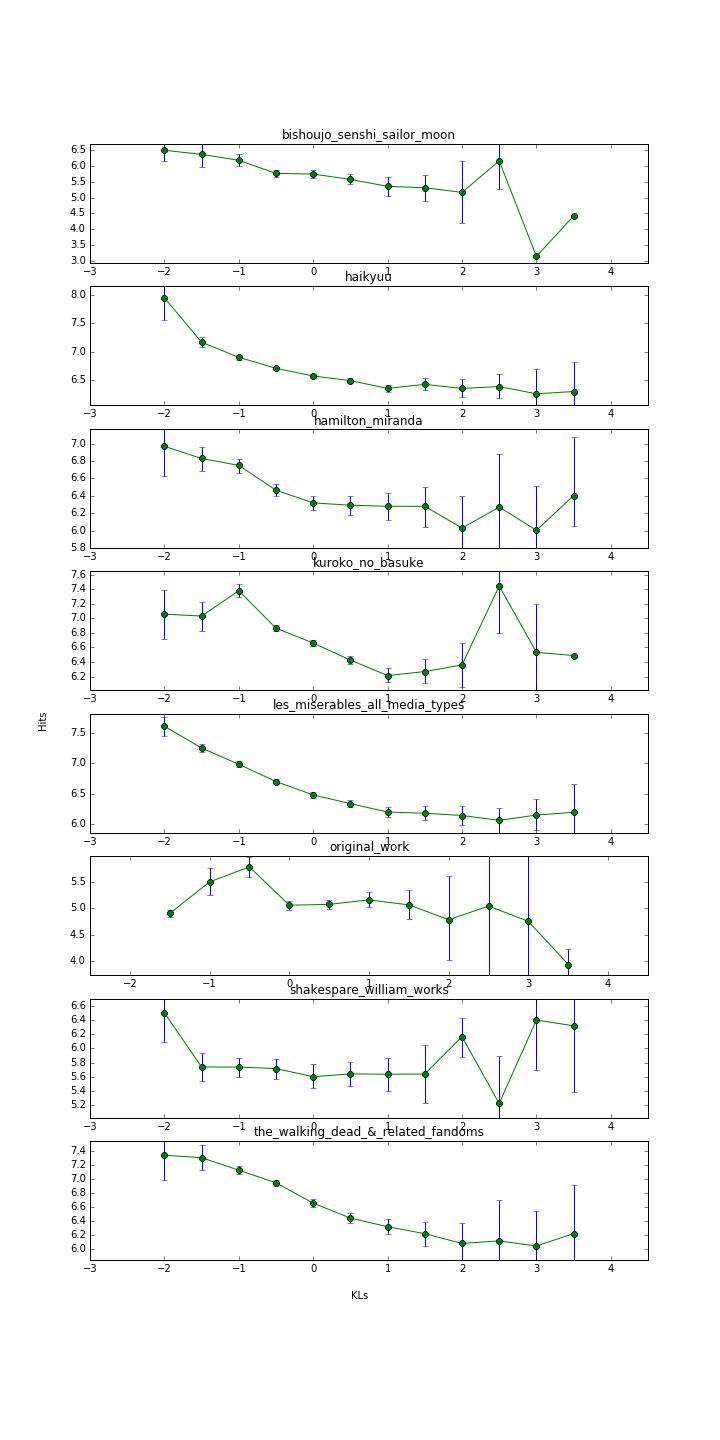
\includegraphics[height=7in]{/kl_hits.png}
        \caption{Hits}
    \end{subfigure}
    \caption{Relation between fictions' KL divergence to standard work and their Kudos or Hits in 8 fandoms. The KL divergence is turned into z-score; both Kudos and Hits are log-transformed. }
    \label{fig:kl_fields}
\end{figure*}










\printbibliography
    
\end{document} %}}}
